\documentclass[../MATH-2000-Notes.tex]{subfiles}
\begin{document}
\chapter{Functions}
\section{Cartesian product}
\textbf{Notation:}
For any objects $x$ and~$y$, mathematicians use $(x,y)$ to denote the \textbf{ordered pair} whose first coordinate is~$x$ and whose second coordinate is~$y$. It is important to know that the order matters: $(x,y)$ is usually not the same as $(y,x)$. (That is why these are called \emph{ordered} pairs. Notice that sets are not like this: sets are unordered, so $\{x,y\}$ \emph{is} always the same as $\{y,x\}$.) It is important to realize that:
\begin{paperbox}{ordered pair}
    $$(x_1,y_1) = (x_2,y_2) \qquad \Leftrightarrow \qquad \text{$x_1 = x_2$ and $y_1 = y_2$}$$
\end{paperbox}
\begin{Definition}
    {Cartesian Product}
    For any sets $A$ and~$B$, we let
    $$ A \times B = \{\, (a,b) \mid a \in A, \ b \in B \,\}
        .$$
    This notation means, for all~$x$, that
    $$ \text{$x \in A \times B$ if and only if $\exists a \in A, \exists b \in B, \ x = (a,b)$.} $$
    The set $A \times B$ is called the \textbf{Cartesian product} of~$A$ and~$B$.
\end{Definition}

\begin{commentbox}{Examples}[{PhbLightCyan}]
    \begin{enumerate}
        \item $\R \times \R = \R^2$.
        \item \label{EasyCartesianEg-123xab}
              $\{1,2,3\} \times \{\text{a}, \text{b} \} =
                  \bigl\{ (1,\text{a}), (1,\text{b}), (2,\text{a}), (2,\text{b}), (3,\text{a}), (3,\text{b}) \bigr\}$.
        \item \label{EasyCartesianEg-abx123}
              $\{\text{a}, \text{b} \} \times \{1,2,3\}  =
                  \bigl\{ (\text{a},1), (\text{a},2), (\text{a},3), (\text{b},1), (\text{b},2), (\text{b},3) \bigr\}$.
    \end{enumerate}
    By comparing \ref{EasyCartesianEg-123xab} and \ref{EasyCartesianEg-abx123}, we see that $\times$ is \emph{not} commutative: $A \times B$ is usually \emph{not} equal to $B \times A$.
\end{commentbox}
\begin{Note}
    {Cardinality of Cardinality Product}
    \label{Card(AxB)Rem}
    We will prove in later that
    $$\#(A \times B) = \#A \cdot \#B .$$
\end{Note}
\begin{proof}[Informal proof]
    Suppose $\#A = m$ and $\#B = n$. Then, by listing the elements of these sets, we may write
    $$ \text{$A = \{a_1,a_2,a_3,\ldots,a_m\}$ \quad and \quad $B = \{b_1,b_2,b_3,\ldots,b_n\}$.} $$
    The elements of $A \times B$ are:
    $$ \begin{matrix}
            (a_1,b_1), & (a_1,b_2), & (a_1,b_3), & \cdots & (a_1,b_n), \\
            (a_2,b_1), & (a_2,b_2), & (a_2,b_3), & \cdots & (a_2,b_n), \\
            (a_3,b_1), & (a_3,b_2), & (a_3,b_3), & \cdots & (a_3,b_n), \\
            \vdots     & \vdots     & \vdots     & \ddots & \vdots     \\
            (a_m,b_1), & (a_m,b_2), & (a_m,b_3), & \cdots & (a_m,b_n)
            .\end{matrix}$$
    In this array,
    \begin{itemize}
        \item each row has exactly $n$ elements, and
        \item there are $m$ rows,
    \end{itemize}
    so the number of elements is the product $m n = \#A \cdot \#B$.
\end{proof}
\begin{Questions}
    \item If A and B are non empty sets, and \(A \times B = B \times A\), then we have \(A = B\).
    \item \label{CartProdDisjoint} If $B$ is disjoint from~$C$, then $A \times B$ is disjoint from $A \times C$.
    \item \label{CartDistribUnionEg} Assume $A$, $B$, and~$C$ are sets. Prove $ A \times (B \cup C) = (A \times B) \cup (A \times C)$.
\end{Questions}
\begin{Answers}
    \item \begin{proof}
        We assume A and B are non-empty sets and \(A \times B = B \times A\). We need to show that \(A \subseteq B\) and \( B \subseteq A\), however, due to symmetry we only need to show that \(A \subseteq B\).

        Let \(a_0 \in A_0\). Since \(B \neq \emptyset\), there exists some \(b_0 \in B\) and we have \((a_0,b_0) \in A \times B = B \times A = \{(b,a); b\in B, a\in A\}\). Hence there exist some \(b \in B\) and \(a \in A\) with \((a_0,b_0) = (a_1,b_1)\), and therefore \(a_0 = b\in B\).
    \end{proof}
    \item  \begin{proof}
        We prove the contrapositive: Assume $A \times B$ is \emph{not} disjoint from $A \times C$, and we will show $B$ is \emph{not} disjoint from~$C$.

        By assumption, the intersection of $A \times B$ and $A \times C$ is not empty, so we may choose some
        $$x \in (A \times B) \cap (A \times C) .$$
        Then:
        \begin{itemize}
            \item Since $x \in A \times B$, there exist $a_1 \in A$ and $b \in B$, such that $x = (a_1,b)$.
            \item Since $x \in A \times C$, there exist $a_2 \in A$ and $c \in C$, such that $x = (a_2,c)$.
        \end{itemize}
        Hence $(a_1,b) = x = (a_2,c)$, so $b = c$.
        Now $b \in B$ and $b = c \in C$, so $b \in B \cap C$. Therefore $B \cap C \neq \emptyset$, so,
        as desired,
        $B$ and~$C$ are \emph{not} disjoint.
    \end{proof}
    \item \begin{proof}
        ($\supset$) Given $x \in (A \times B) \cup (A \times C)$, we have $x \in A \times B$ or $x \in A \times C$. By symmetry, we may assume $x \in A \times B$, so $x = (a,b)$ for some $a \in A$ and $b \in B$. Note that $b \in B \cup C$, so we have $a \in A$ and $b \in B \cup C$. Therefore
        $$ x = (a,b) \in A \times (B \cup C) .$$
        Since $x$ is an arbitrary element of $(A \times B) \cup (A \times C)$, this implies $ (A \times B) \cup (A \times C) \subset A \times (B \cup C)$.

        ($\subset$) Given $(a,x) \in A \times (B \cup C)$, we have $a \in A$, and either $x \in B$ or $x \in C$. By symmetry, we may assume $x \in B$. Then $(a,x) \in A \times B \subset (A \times B) \cup (A \times C)$, so $(a,x) \in (A \times B) \cup (A \times C)$.
        Since $(a,x)$ is an arbitrary element of $A \times (B \cup C)$, this implies $A \times (B \cup C) \subset (A \times B) \cup (A \times C)$.
    \end{proof}
\end{Answers}

\section{Informal Introduction to Functions}
Ever since junior high you have seen functions in the form of a formula i.e., \(f(x)  = x^2\). However there are other ways to define a function. The key property of a function is that it accepts inputs, and provides a corresponding output value for each possible input.

\begin{Definition}
    {Informal Def of a Functions}
    Suppose $f$ is any function.
    \begin{enumerate}
        \item The set of allowable inputs of $f$ is called the \textbf{domain} of~$f$.
        \item If $A$ is the domain of~$f$, and $B$~is any set that contains all of the possible outputs of~$f$, then we say that $f$ is a \textbf{function from~$A$ to~$B$}. In the case of the function $f(x) = x^3$, we may take $A$ and~$B$ to both be the set of real numbers; thus, $f$~is a function from~$\real$ to~$\real$.
    \end{enumerate}
\end{Definition}

\subsection{Ways to describe a function}
There are many ways to describe a function
\begin{enumerate}
    \item A table\\
          \begin{tabular}{l|l}
              \textbf{item} & \textbf{price in cents} \\
              apple         & 65                      \\
              banana        & 83                      \\
              cherry        & 7                       \\
              \vdots        & \vdots
          \end{tabular}
    \item A set of ordered pairs: The price function would be represented as : \(\{(Apple, 65),(Banana, 83),(Cherry, 7),\dots\}\)
    \item An arrow diagram: we can also do this \(f: A\rightarrow B\)
          \begin{itemize}
              \item A dot is drawn for each element in set A and B
              \item An arrow is drawn from a to f(a), for each \(a\in A\).
          \end{itemize}
\end{enumerate}

\section{Official Functions}
\begin{Definition}
    {Function}
    Suppose $A$ and~$B$ are sets.
    \begin{enumerate}
        \item \label{FunctionDefn-func}
              A set~$f$ is a
              \textbf{function from~$A$ to~$B$} if and only if
              \begin{enumerate}
                  \item \label{FunctionDefn-func-pair}
                        each element of~$f$ is an ordered pair $(a,b)$, such that $a \in A$ and $b \in B$,
                        and
                  \item \label{FunctionDefn-func-unique}
                        for each $a \in A$, there is a \emph{unique} $b \in B$, such that $(a,b) \in f$.
              \end{enumerate}
        \item If $f$ is a function from~$A$ to~$B$, then
              \begin{itemize}
                  \item $A$ is called the \textbf{domain} of~$f$,
                        and
                  \item $B$ is a \textbf{codomain} of~$f$.
              \end{itemize}
        \item We write ``$f \colon A \to B$''%
              to denote that $f$ is a function from~$A$ to~$B$.
    \end{enumerate}

\end{Definition}
\begin{Note}
    we write \(f(a) = b\) if and only if \((A,b)\in f\).
\end{Note}
\begin{Definition}
    {Range}
    Let \(f:A\rightarrow B\), then the range of f is the set \(\{f(a);a\in A\}\).
\end{Definition}

\section{One-to-One Functions}
\begin{Definition}
    {One-to-One function}
    Suppose \(f:A\rightarrow B\) we say \(f:A\rightarrow B\) is \textbf{one-to-one} or (injective) if and only if \(\forall a_1,a_2\in A; f(a_1) = f(a_2) \Rightarrow a_1 = a_2\)
\end{Definition}
\begin{commentbox}{Example}[{PhbLightCyan}]
    Let \(F: \R \rightarrow \R\), be defined as \(f(x) x^2\). Then f is not one-to-one, since \(f(2) = 2^2 = 4 = (-2^2) = f(-2)\) but \(2 \neq -2\).
\end{commentbox}
\begin{figure}[h]
    \centering
    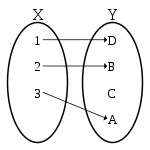
\includegraphics[width=0.6\columnwidth]{../Assets/150px-Injection.svg.png}
    \caption{one-to-one functions}
    \label{fig:1to1}
\end{figure}
\begin{commentbox}{Example}[{PhbLightCyan}]
    Prove that \(f(x) = x + 1\) is one-to-one
\end{commentbox}
\begin{proof}
    let \(x_1,x_2 \in \R\) such that \(f(x_1) = f(x_2)\). Then we have \(x_1 + 1 = x_2 + 1\) hence \(x_1 = x_2\) as desired.
\end{proof}
\begin{Theorem}
    {}\label{alternate11thm}
    If a function $f\colon A \to B$ is one-to-one, then $$\forall a_1, a_2 \in A, \bigl( a_1 \neq a_2 \Rightarrow f(a_1) \neq f(a_2)\bigr).$$
\end{Theorem}
\begin{proof}
    Let $f \colon A \to B$ be one-to-one. Given $a_1,a_2 \in A$, we know, from the definition of one-to-one,  that
    $$  f(a_1) = f(a_2) \Rightarrow a_1 = a_2 .$$
    So the contrapositive of this implication is also true. That is,
    \[
        a_1 \neq a_2 \Rightarrow f(a_1) \neq f(a_2) .
    \]
\end{proof}

\section{Onto Functions}
\begin{Definition}
    {Onto Function}
    Suppose $f \colon A \to B$. We say $f$ is \textbf{onto} if and only if, for all $b \in B$, there is some $a \in A$, such that $f(a) = b$.
\end{Definition}
\begin{figure}[h]
    \centering
    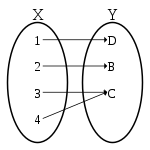
\includegraphics[width=0.6\columnwidth]{../Assets/150px-Surjection.svg.png}
    \caption{Onto}
    \label{fig:onto}
\end{figure}

\begin{commentbox}{Example}[{PhbLightCyan}]
    \(f:\R\rightarrow \R\) be \(f(x) =  |x|\) prove that its not onto.
\end{commentbox}
\begin{proof}
    Note that \(-1 \in \R\). Then \(f(x) = |-1| = 1 \geq 0 > -1\), so there does not exist \(x \in \R\) for which \(f(x) = -1\) hence f is not onto.
\end{proof}
\section{Bijection}
\begin{Definition}
    {Bijection}
    We say a function has a bijection if and only if the function is one-to-one \textbf{and} onto.

    Moreover, if the function \(f: A \rightarrow B\) then the two sets A and B must have exactly the same number of elements.
\end{Definition}
\begin{figure}[h]
    \centering
    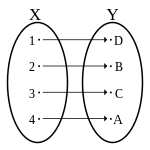
\includegraphics[width=0.6\columnwidth]{../Assets/150px-Bijection.svg.png}
    \caption{Bijection}
    \label{fig:bijection}
\end{figure}
\begin{Note}
    Let \(f: A \rightarrow B\) we have the following
    \begin{enumerate}
        \item If f is one-to-one, then each element of A gets mapped to a unique element of B. Therefore, \(\#A \leq \#B\).
        \item If f is onto, then all elements of B is mapped to at least one element from A. Therefore, \(\#A \geq \#B\).
    \end{enumerate}
\end{Note}
In general to prove a function \(f: A\rightarrow B\) that is
\begin{enumerate}
    \item one-to-one, we let \(a_1,a_2 \in A\) for which \(f(a_1) = f(a_2) \Rightarrow a_1 = a_2\).
    \item Not one-to-one, we provide a counterexample
    \item onto, we prove that \(\forall b \in B, \exists a \in A\) such that \(f(a) = b\).
    \item not onto, we provide a counterexample where given a element from B there does not exist an element from A such that \(f(a) = b\).
\end{enumerate}
\begin{Definition}
    {Identity map}
    or any set~$A$, define the \textbf{identity map} $I_A \colon A \to A$ by $I_A(a) = a$ for every $a \in A$.
\end{Definition}
\begin{commentbox}{Example}[{PhbLightCyan}]
    Let \(f: \R \rightarrow \R\) be defined by \(f(x) = 7x - 3\). Prove f is a bijection.
\end{commentbox}
\begin{proof}~\\
    (one-to-one) Set \(x_1,x_2 \in \R\) and assume that \(f(x_1) = f(x_2)\) then we have , \(7x_1 - 3 = 7x_2 - 3 \Rightarrow 7x_1 = 7x_2 \Rightarrow x_1 = x_2\), therefore f is one-to-one.

    (onto) Given \(y \in \R\), let \(x = \frac{y + 3}{7} \in \R\). Then we have
    \begin{gather*}
        f(x) = 7x-3\\
        = 7 \left( \frac{y + 3}{7} \right)-3\\
        = y + 3 - 3\\
        = y
    \end{gather*}
    Since y was arbitrary we conclude that f is onto

    Since f is both one-to-one and onto we conclude that f is bijective by definition.
\end{proof}
\section{Inverse Function}
\begin{Definition}
    {Inverse Function}
    Suppose
    \begin{itemize}
        \item $f \colon A \to B$,
              and
        \item $g \colon B \to A$.
    \end{itemize}
    We say that $g$ is the \textbf{inverse} of~$f$ if and only if:
    \begin{enumerate} \renewcommand{\theenumi}{\alph{enumi}}
        \item $g \bigl( f(a) \bigr) = a$ for all $a \in A$,
              and
        \item $f \bigl( g(b) \bigr) = b$ for all $b \in B$.
    \end{enumerate}

    The inverse of the function f is denoted by \(f^{-1}\)  \[f^{-1}(x) = \frac{1}{f(x)}\]
\end{Definition}
\begin{figure}[htbp]
    \centering
    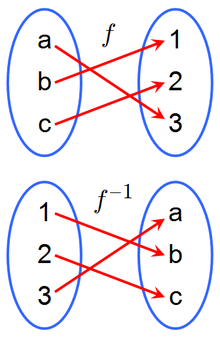
\includegraphics[width=0.6\columnwidth]{../Assets/220px-Inverse_Function.png}
    \caption{Inverse}
    \label{fig:inverse}
\end{figure}
\newpage
\begin{commentbox}{Example}[{PhbLightCyan}]
    Let \(f: \R \rightarrow \R\) be defined by \(f(x) = 7x - 4\), and let \(g: \R \rightarrow \R\) be defined by \(g(x) = \frac{x + 4}{7}\). Prove that g is the inverse of f.
\end{commentbox}
\begin{proof}
    it suffice to show two things
    \begin{enumerate}
        \item \(g(f(x)) = x\ \ \forall x \in \R\)
        \item \(f(g(y)) = y\ \ \forall y \in \R\)
    \end{enumerate}
    ~\\
    \begin{enumerate}
        \item Let \(x \in \R \). Then we have \(g(f(x)) = \frac{f(x) + 4}{7} = \frac{(7x - 4) + 4 }{7}\)
        \item Let \(y \in \R \). Then we have \(f(g(y)) = 7g(y) - 4 = 7\left( \frac{y + 4}{7} \right) - 4 = y + 4 - 4 = y\)
    \end{enumerate}
\end{proof}
\begin{Theorem}
    {}\label{Inverse->Bijection}
    Suppose $f\colon A \to B$. If $f$ has an inverse $f^{-1} \colon B \to A$, then $f$ is a bijection.
\end{Theorem}



\section{Composition of a Function}
\begin{Definition}
    {Composition of a Function}
    Suppose that \(f: A\rightarrow B\) and \(g: B \rightarrow C\) the composition of g and f is the function gof. \(gof: A \rightarrow C\), defined by \(gof(x) = g(f(a))\)
\end{Definition}
Define $f \colon \R \to \R$ and $g \colon \R \to \R$ by
$f(x) = 3x$ and $g(x) = x^2$. Then $g \circ f$ and $f \circ g$ are functions from~$\R$ to~$\R$. For all $x \in \R$, we have
$$(g \circ f)(x) = g \bigl( f(x) \bigr) = g(3x) =(3x)^2 =  9x^2 $$
and
$$(f \circ g)(x) = f \bigl( g(x) \bigr) = f(x^2) = 3(x^2) = 3x^2 .$$
Notice that (in this example) $f \circ g \neq g \circ f$, so \emph{composition is \textbf{not} commutative}.

\begin{Proposition}
    {}
    Let \(f: A \rightarrow B\) and let \(f^{-1}: B \rightarrow A\) be the inverse of f. Then, we have \begin{enumerate}
        \item \(f^{-1} \circ f = I_A\)
        \item \(f \circ f^{-1} = I_B\)
    \end{enumerate}
\end{Proposition}

\begin{commentbox}{Example}[{PhbLightCyan}]\label{ComposegBijEg}
    Suppose $f \colon A \to B$ and $g \colon B \to C$. Show that if $f$ and $g \circ f$ are bijections, then $g$ is a bijection.
\end{commentbox}

\begin{proof}
    It suffices to show that $g$ is both one-to-one and onto.

    (one-to-one) Let $b_1$ and $b_2$ be arbitrary elements of~$B$, such that $g(b_1) = g(b_2)$. Since $f$ is a bijection, it is onto, so there exist $a_1,a_2 \in A$, such that $f(a_1) = b_1$ and $f(a_2) = b_2$. Then
    $$ (g\circ f)(a_1) = g\bigl( f(a_1) \bigr) = g(b_1) = g(b_2) =g \bigl( f(a_2) \bigr) = (g \circ f)(a_2) .$$
    Since $g \circ f$ is a bijection, it is one-to-one, so we conclude that $a_1 = a_2$. Therefore
    $$ b_1 = f(a_1) = f(a_2) = b_2 .$$
    Since $b_1$ and~$b_2$ are arbitrary elements of~$B$, such that $g(b_1) = g(b_2)$, this implies that $g$ is one-to-one.

    (onto) Let $c$ be an arbitrary element of~$C$. Since $g \circ f$ is a bijection, it is onto, so there exists $a \in A$, such that $(g \circ f)(a) = c$. Let $b = f(a)$. Then
    $$ g(b) = g \bigl( f(a) \bigr) = (g \circ f)(a) = c .$$
    Since $c$ is an arbitrary element of~$C$, we conclude that $g$ is onto.
\end{proof}


\section{Image and Preimage}
\begin{Definition}
    {Image}
    Suppose $f \colon A \to B$, and $A_1 \subset A$. The \textbf{image} of $A_1$ under~$f$ is
    $$ f(A_1) = \{f(a);\ a\in A_!\} \subseteq B $$
    It is a subset of~$B$. The notation means that, for all~$x$, we have
    $$ x \in f(A_1) \quad \Leftrightarrow \quad \exists a \in A_1, \bigl( x = f(a) \bigr) .$$
\end{Definition}
\begin{commentbox}{Example}[{PhbLightCyan}]
    Assume $f \colon A \to B$.
    Show that if $A_1$ and~$A_2$ are subsets of~$A$, and $f$ is one-to-one, then \  $f(A_1) \cap f(A_2) \ \subset \ f(A_1 \cap A_2)$.
\end{commentbox}
\begin{proof}
    Given $b \in f(A_1) \cap f(A_2)$, we know $b \in f(A_1)$ and $b \in f(A_2)$. Therefore, since $b \in f(A_1)$, we know there is some $a_1 \in A_1$, such that $b = f(a_1)$. Also, since $b \in f(A_2)$, we know there is some $a_2 \in A_2$, such that $b = f(a_2)$. Then
    $$ f(a_1) = b = f(a_2) .$$
    Since $f$ is one-to-one, this implies $a_1 = a_2 \in A_2$. Since we also know that $a_1 \in A_1$, this implies $a_1 \in A_1 \cap A_2$. So $f(a_1) \in f(A_1 \cap A_2)$. Since $b = f(a_1)$, this means $b \in f(A_1 \cap A_2)$. Since $b$ is an arbitrary element of $f(A_1) \cap f(A_2)$, we conclude that $f(A_1) \cap f(A_2) \subset f(A_1 \cap A_2)$.
\end{proof}
\begin{Definition}
    {Preimage}
    Suppose $f \colon A \to B$, and $B_1 \subset B$. The \textbf{pre-image} (or \textbf{inverse image}) of $B_1$ under~$f$ is
    $$ f^{-1}(B_1) = \{\forall a\in A; f(a) \in B_1\} \subseteq A.$$
    It is a subset of~$A$. When $B_1 = \{b\}$ has only one element, we usually write $f^{-1}(b)$, instead of $f^{-1} \bigl( \{b\} \bigr)$.
\end{Definition}

\begin{commentbox}{Example}[{PhbLightCyan}]
    Suppose $f \colon A \to B$ and $B_1 \subset B$.
    \begin{multicols}{2}
        \begin{enumerate}
            \item \label{InvImgContainEg-f(f(B1))inB1}
                  We have $f \bigl( f^{-1}(B_1) \bigr) \subset B_1$.
            \item \label{InvImgContainEg-f(f(B1))=B1}
                  If $f$ is onto, then $f \bigl( f^{-1}(B_1) \bigr) = B_1$.
        \end{enumerate}
    \end{multicols}
\end{commentbox}

\begin{proof}
    \ref{InvImgContainEg-f(f(B1))inB1} Let $b \in f \bigl( f^{-1}(B_1) \bigr)$. By definition, we have
    $$ f \bigl( f^{-1}(B_1) \bigr) = \{ f(a); a \in f^{-1}(B_1) \} ,$$
    so we must have $b =  f(a_1)$, for some $a_1 \in f^{-1}(B_1)$. From the definition of $f^{-1}(B_1)$, we know that $f(a_1) \in B_1$. Therefore $b = f(a_1) \in B_1$. Since $b$ is an arbitrary element of $f \bigl( f^{-1}(B_1) \bigr)$, this implies that $f \bigl( f^{-1}(B_1) \bigr) \subset B_1$, as desired.

    \smallskip
    \ref{InvImgContainEg-f(f(B1))=B1} Assume $f$ is onto. We know, from~\ref{InvImgContainEg-f(f(B1))inB1}, that $f \bigl( f^{-1}(B_1) \bigr) \subset B_1$, so it suffices to show that $B_1 \subset f \bigl( f^{-1}(B_1) \bigr)$.

    Let $b \in B_1$ be arbitrary. Because $f$ is onto, we know there exists $a_1 \in A$, such that $f(a_1) = b$. Then $f(a_1) = b \in B_1$, so $a_1 \in  f^{-1}(B_1)$. Therefore
    $$ f(a_1) \in \{ f(a); a \in f^{-1}(B_1) \} = f \bigl( f^{-1}(B_1) \bigr) .$$
    Since $f(a_1) = b$, we conclude that $b \in f \bigl( f^{-1}(B_1) \bigr)$.
    Since $b$ is an arbitrary element of~$B_1$, this implies that $B_1 \subset f \bigl( f^{-1}(B_1) \bigr)$, as desired.
\end{proof}

\end{document}